\documentclass{article}
\usepackage[utf8]{inputenc}
\usepackage{geometry}
\usepackage{siunitx}
\usepackage{amsmath,amsfonts,amssymb}
\usepackage{nccmath}
\usepackage{multicol}
\usepackage{chngcntr}
\usepackage{mathtools}
\usepackage{float}
\usepackage{xspace}
\usepackage{chngcntr}
\usepackage[super]{nth}
\usepackage[section,above,below]{placeins}
\usepackage{hyperref}
\usepackage{caption}
\usepackage{subcaption}

\geometry{
    a4paper,
    left    = 40mm,
    right   = 40mm,
    top     = 40mm,
    bottom  = 40mm,
}

\begin{document}

\begin{titlepage}
	\centering
	\vspace{5cm}
	{\scshape\Huge Delft University of Technology \par}
	\vspace{1.5cm}
	{\scshape\Large AE4313-20 Spacecraft Attitude Dynamics and Control Project\par}
    
	\vspace{\fill}
	\flushleft
	{\scshape\large\begin{tabular}{@{}ll}
	    Students:       & Thomas Nagy Zambo 5140196 \\
	    Instructors:    & Dr. ir. E. van Kampen \\
	\end{tabular}\par}
	\vspace{0.5cm}
    
                        
    {\scshape\large June \nth{9}, 2023\par}
\end{titlepage}

\newgeometry{
    left    = 30mm,
    right   = 30mm,
    top     = 30mm,
    bottom  = 30mm,
}

\pagenumbering{roman}


\tableofcontents
\listoffigures
\section*{Code}
\url{https://github.com/tnagyzambo/AE4313-Project}

\newpage
\pagenumbering{arabic}
\setcounter{page}{1}

\section{Introduction}

The goal of this assignment is to create a control system for the attitude tracking problem of a Nadir pointing spacecraft. This control system is robust to external disturbances as well as noise and bias in the sensor measurements. To achieve this, the control system consists of a PD controller and a Multiplacative Quaternion Extended Kalman Filter (MQEFK). In order to further explore the problem space, additional goals were set beyond what were outlined in the assignment. Firstly, the code used simulate the satellite is written in Rust in order to gain an understanding of the practical challenges involved with writting production quality simulations software in a systems-level language. The code created for this assignment might not meet the bar of `production quality`, but a significant amount of understanding was gained in the attempt. Second, the LVLH frame of the circular orbit is modelled and the full Nadir tracking problem of aligning the body axes to the rotating LVLH reference frame is considered. Third, where ever possible quaternions are used to model the system in order to develop a deeper understanding about the math behind them.

\section{Simulation Framework}

An adaptive time-stepping Runge-Kutta 45 (RK45) solver was written and used to simulate all results in this assigment.The motivation for using an RK45 is the proven peformance of the algorithm. The selection of adaptive-time stepping is motivated by the potential for long running space missions with protions of low dynmic intesitty. Taking larger time steps in these areas can siginifcantly reduce the computational cost. However the control loop must run at a fixed interval, so additional logic must be included in the RK45 solver to not overrun the next iteration of the control loop. The main logic of this selection between adaptive stepping and fixed interval control can be found in Figure \ref{fig:main_loop}.

\begin{figure}[h]
	\begin{verbatim}
    while t < t_end {
        let (x_new, dt_new) = solver.step(x, u, df, t, dt);

        let t_next_control_step = t_prev_control_step + dt_control;

        if (t + dt) > t_next_control_step {
            (x, dt) = solver.step_to(x, u, df, t, t_next_control_step);
            t = t + dt;
            u = controller.step(x);
            t_prev_control_step = t;
        } else {
            t = t + dt;
            x = x_new;
        }
        dt = dt_new;
    }
	\end{verbatim}
	\caption{Adaptive Time-stepping with Fixed Control Interval Logic}
	\label{fig:main_loop}
\end{figure}

\section{Building the Model}

\subsection{Orbits and Reference Frames}

The Earth Centered Inertial (ECI) reference frame $\mathcal{F}_I$ is placed coincedent to the basis of the cartesian coordinates system. The position and velocty of the spacecraft w.r.t. $\mathcal{F}_I$ are defined by $\vec{r}$ and $\vec{v}$ respectivley. From this, the kinematics (\ref{eqn:kin_orbit}) and dynamics (\ref{eqn:dyn_orbit}) for a simple circular orbit can be written. These values are initialized with a $\vec{r}$ and $\vec{v}$ corresponding to a 700km orbit at an arbitrary inclication.

\begin{equation}
	\dot{r} = \frac{\vec{r} \times \vec{v}}{|\vec{r}|^2} \times \vec{r}
	\label{eqn:kin_orbit}
\end{equation}

\begin{equation}
	\dot{v} = \left|\frac{\vec{r} \times \vec{v}}{|\vec{r}|^2}\right|^2 \vec{r} 
	\label{eqn:dyn_orbit}
\end{equation}

The Local Vertical Local Horizon (LVLH) refernce frame $\mathcal{F}_{L}$ can be built from these vectors by creating the quaternion $q_{L}$ (\ref{eqn:q_lvlh}) that rotates $\mathcal{F}_I$ to $\mathcal{F}_{L}$. This is done by creating a quaternion $q_1$ (\ref{eqn:q1}) that rotates the $\hat{k}$ vector of the basis to align with $\vec{r}$. A second quaternion $q_2$ (\ref{eqn:q2}) is then created to rotate the transformed basis about its $\hat{k}$ axis. The angle of this rotation is equal to the dot product of the transformed $\hat{i}$ direction and $\vec{v}$. Since the dot product operator provides no indication of the direction of rotation, only the magnitude, some logic is used to correctly rotate the basis.

\begin{equation}
	q_1 = [1 + \hat{k} \times -\hat{r}, [\hat{k} \times -\hat{r}]^T]^T
	\label{eqn:q1}
\end{equation} 

\begin{equation}
\begin{aligned}
	q2 &= \left[\cos\left(\frac{\theta}{2}\right), \left[\sin\left(\frac{\theta}{2}\right) * \hat{r}\right]^T\right]^T \\
	\theta &= \textrm{sign}\left(\sin^{-1}\left(\left[\left(q_1 \otimes \hat{i} \otimes q_1^{-1}\right) \times \hat{v} * \hat{r}^T\right] * \hat{i}\right)\right)\frac{\cos^{-1}\left(\left(q_1 \otimes \hat{i} \otimes q_1^{-1}\right) \cdot \hat{v}\right)}{2} \\ \end{aligned}
	\label{eqn:q2}
\end{equation}

\begin{equation}
	q_{\textrm{L}} = q_2 \otimes q_1
	\label{eqn:q_lvlh}
\end{equation}

To determine correct functioning of the orbit, the LVLH frame transformation over time is simulated. This formulation of the LVLH frame contained a discontinuity in the quaternion that pervents smooth control of the spacecraft over multiple orbits. This issues was not able to be solved within the time constraints of the project. Figures \ref{fig:quat_lvlh} and \ref{fig:orbit_lvlh} show the evolution over time of $q_L$ and the correct functioning of the $\mathcal{F}_L$ simulation. Due to the disconinity futher sections will only consider a partial orbit.

\begin{figure}[H]
\centering
	\begin{subfigure}[b]{0.6\textwidth}
		\centering
		\includegraphics[width=8cm]{images/lvlh_attitude.png}
		\caption{Evolution of $q_{L}$}
		\label{fig:quat_lvlh}
	\end{subfigure}
	\begin{subfigure}[b]{0.3\textwidth}
		\centering
		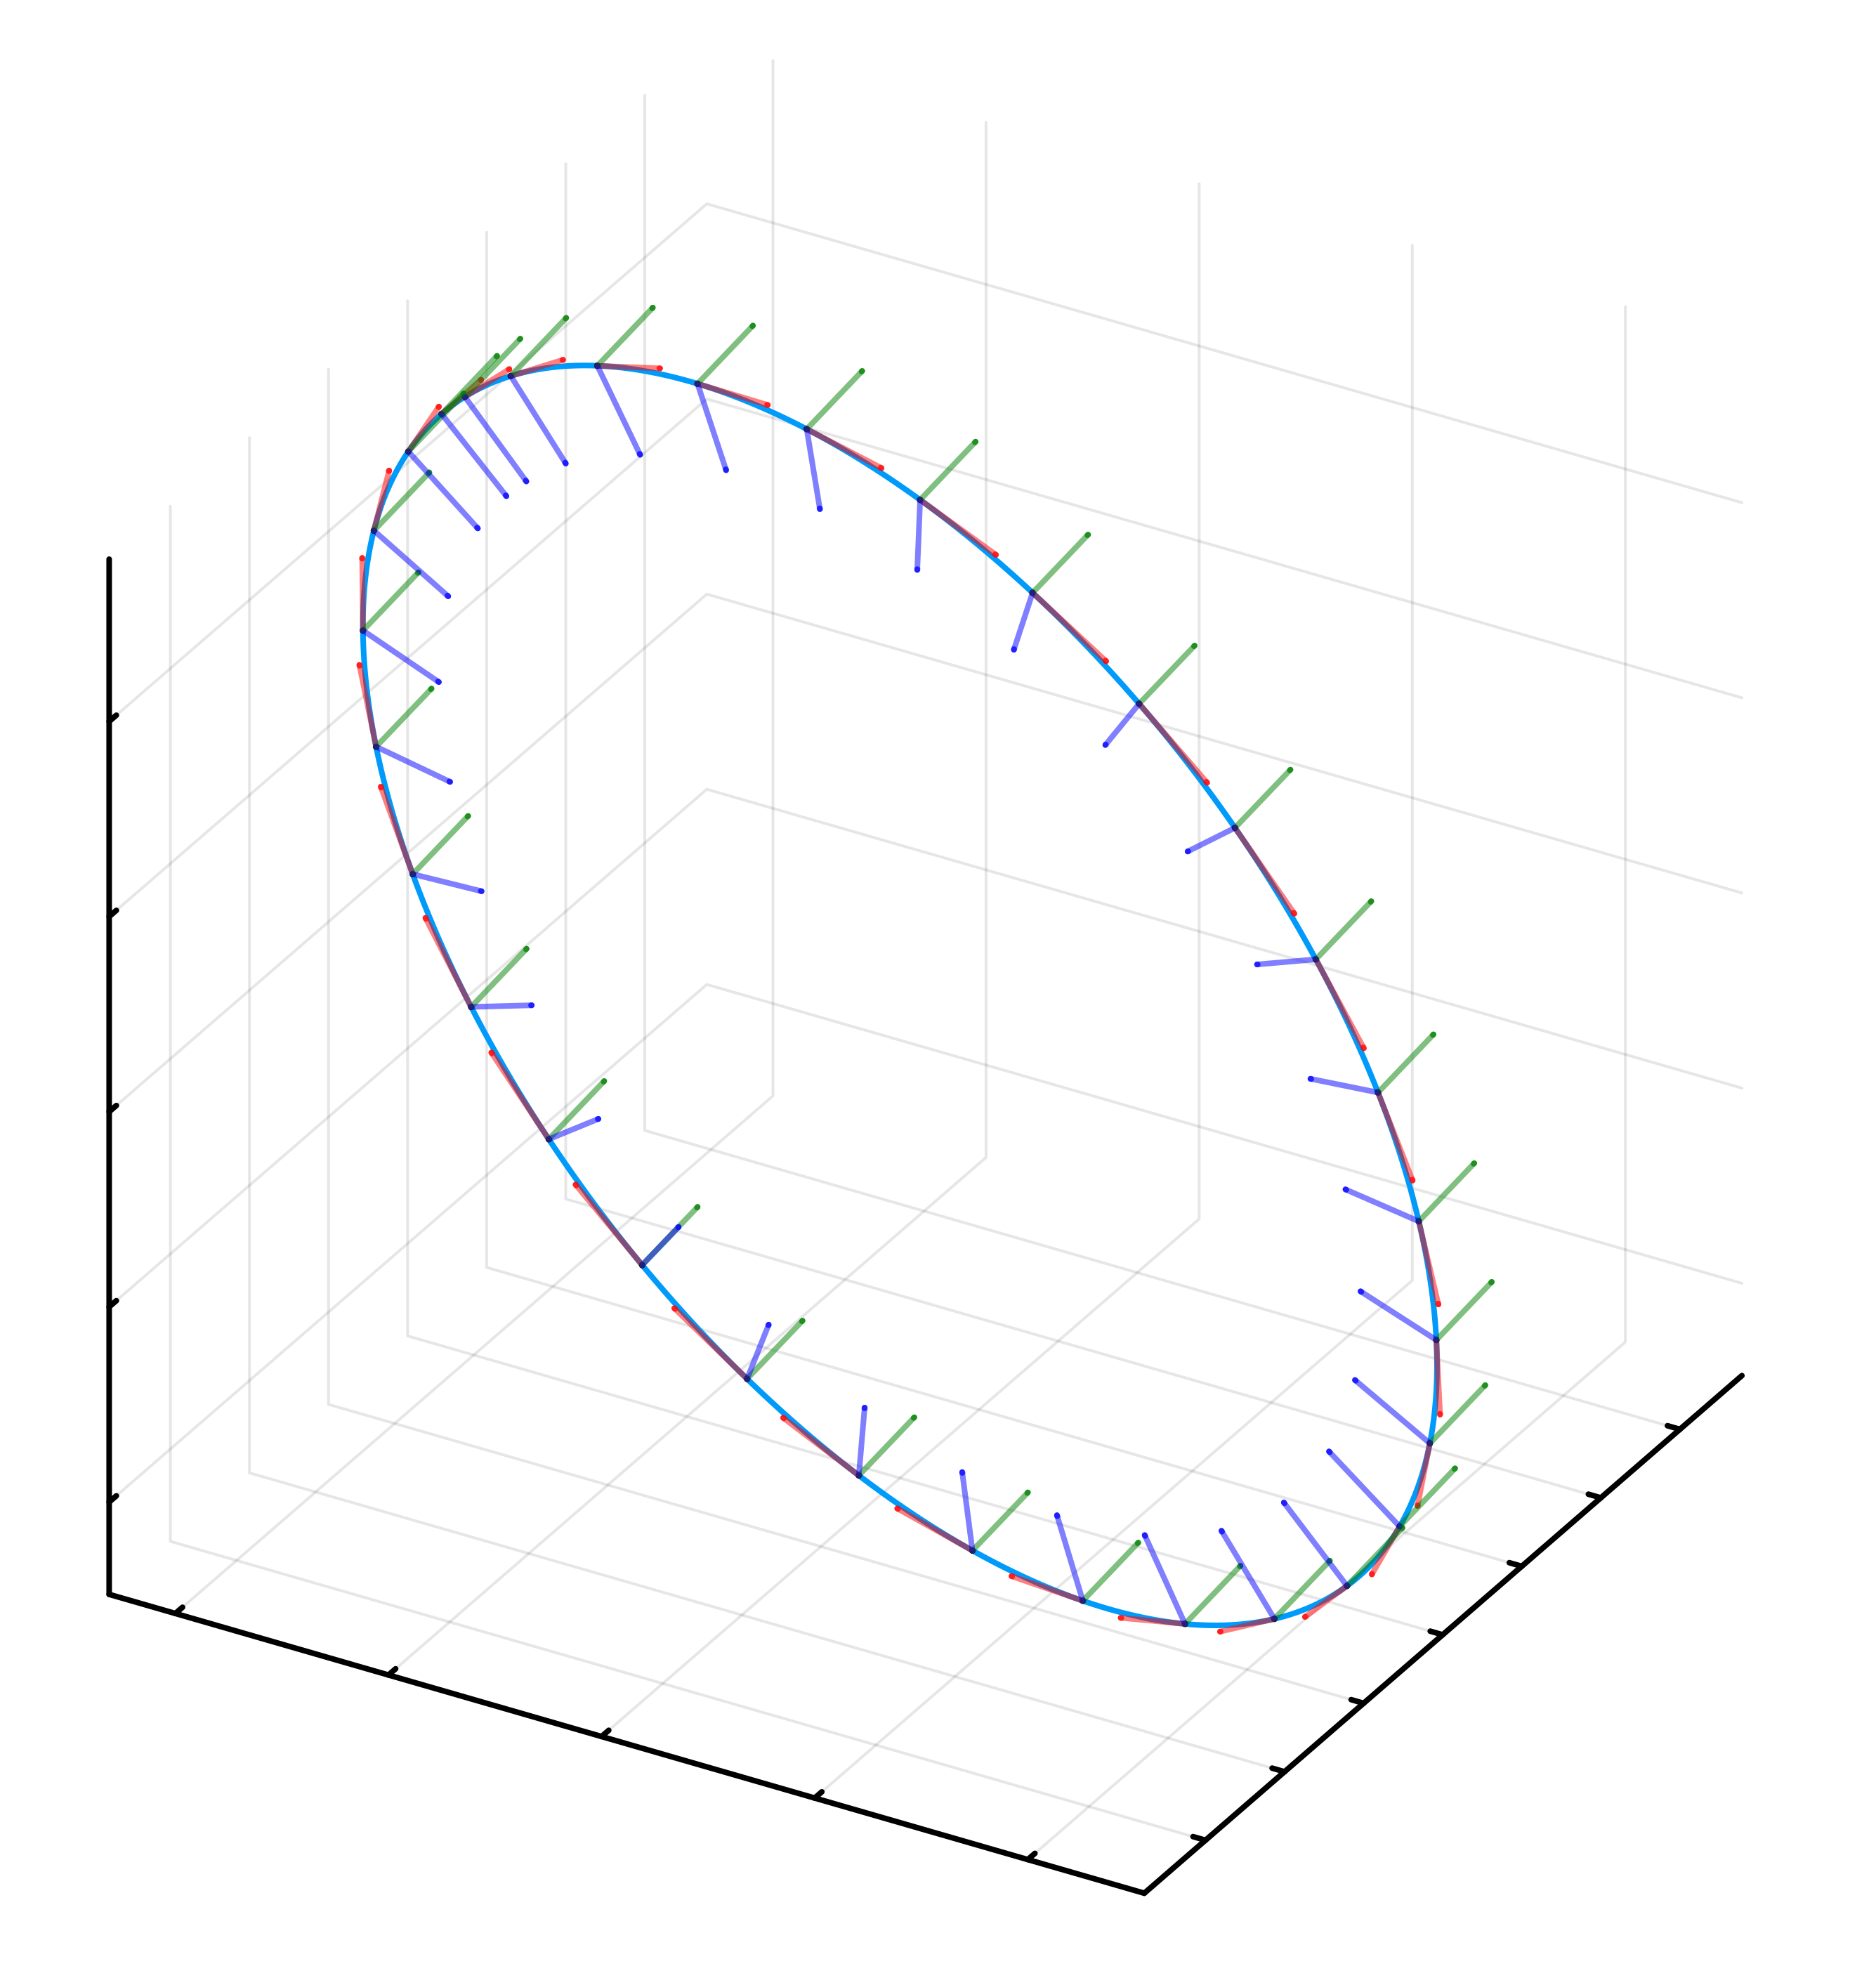
\includegraphics[width=4cm]{images/lvlh_orbit_0s_to_6100s.png}
		\caption{Evolution of $\mathcal{F}_{L}$}
		\label{fig:orbit_lvlh}
	\end{subfigure}
	\caption{LVLH Reference Frame Simulation}
\end{figure}

\subsection{Sattelite Model}

The sattelite kinematics \ref{eqn:kin_sat} and dynamics \ref{eqn:dyn_sat} are modelled in quaterion form. The equations describe the motion of the sattilite's body reference frame $\mathcal{F}_B$ with respect to $\mathcal{F}_I$. The quaternion $q_{B/I}$ decribes the rotation from $\mathcal{F}_I$ to $\mathcal{F}_B$ while the vector $\omega_{B/I}^B$ describes the agular velocity of $\mathcal{F}_B$ with respect to $\mathcal{F}_I$ expressed in $\mathcal{F}_B$. 

\begin{equation}
	\dot{q}_{B/I} = \frac{1}{2} \omega_{B/I}^B \otimes q_{B/I}
	\label{eqn:kin_sat}
\end{equation}

\begin{equation}
	\dot{\omega}_{B/I}^{B} = I^{-1} \left(-\omega_{B/I}^B \times I\omega_{B/I}^B + T_{gg} + T_{dist} + u\right)
	\label{eqn:dyn_sat}
\end{equation}

The inertial matrix of the sattelite $I$ \ref{eqn:inertia} and the disturbance torque $T_{dist}$ \ref{eqn:t_dist} are implemented with the values from the assignment.

\begin{equation}
	I = \left[\begin{matrix}
		2500 & 0    & 0 \\
		0    & 2300 & 0 \\
		0    & 0    & 3100 \\
	\end{matrix}\right] \SI{}{\kilogram\meter^2}
	\label{eqn:inertia}
\end{equation}

\begin{equation}
	T_{dist} = \left[\begin{matrix}
		0.001 & 0.001 & 0.001
	\end{matrix}\right]^T \SI{}{\newton\meter}
	\label{eqn:t_dist}
\end{equation}

The gravity gradient torque experianced by the satellite is implemented as a function of it's orbital position $\vec{r}$ \ref{eqn:t_gg}.

\begin{equation}
	T_{gg} = \frac{3\mu}{|\vec{r}|^3} -\hat{r} \times (-I\hat{r}) \SI{}{\newton\meter}
	\label{eqn:t_gg}
\end{equation}

Simulating the satellite with and inital \SI{10}{\degree} error with respect to $\mathcal{F}_L$ on all body axes results in the motion seen in Figures \ref{fig:quat_dist} and \ref{fig:orbit_dist}. As expected the satellite slowly begins to tumble and by then of the first orbit has completley destabilized.

\begin{figure}[H]
\centering
	\begin{subfigure}[b]{0.6\textwidth}
		\centering
		\includegraphics[width=8cm]{images/dist_attitude.png}
		\caption{Evolution of $q_{B/I}$}
		\label{fig:quat_dist}
	\end{subfigure}
	\begin{subfigure}[b]{0.3\textwidth}
		\centering
		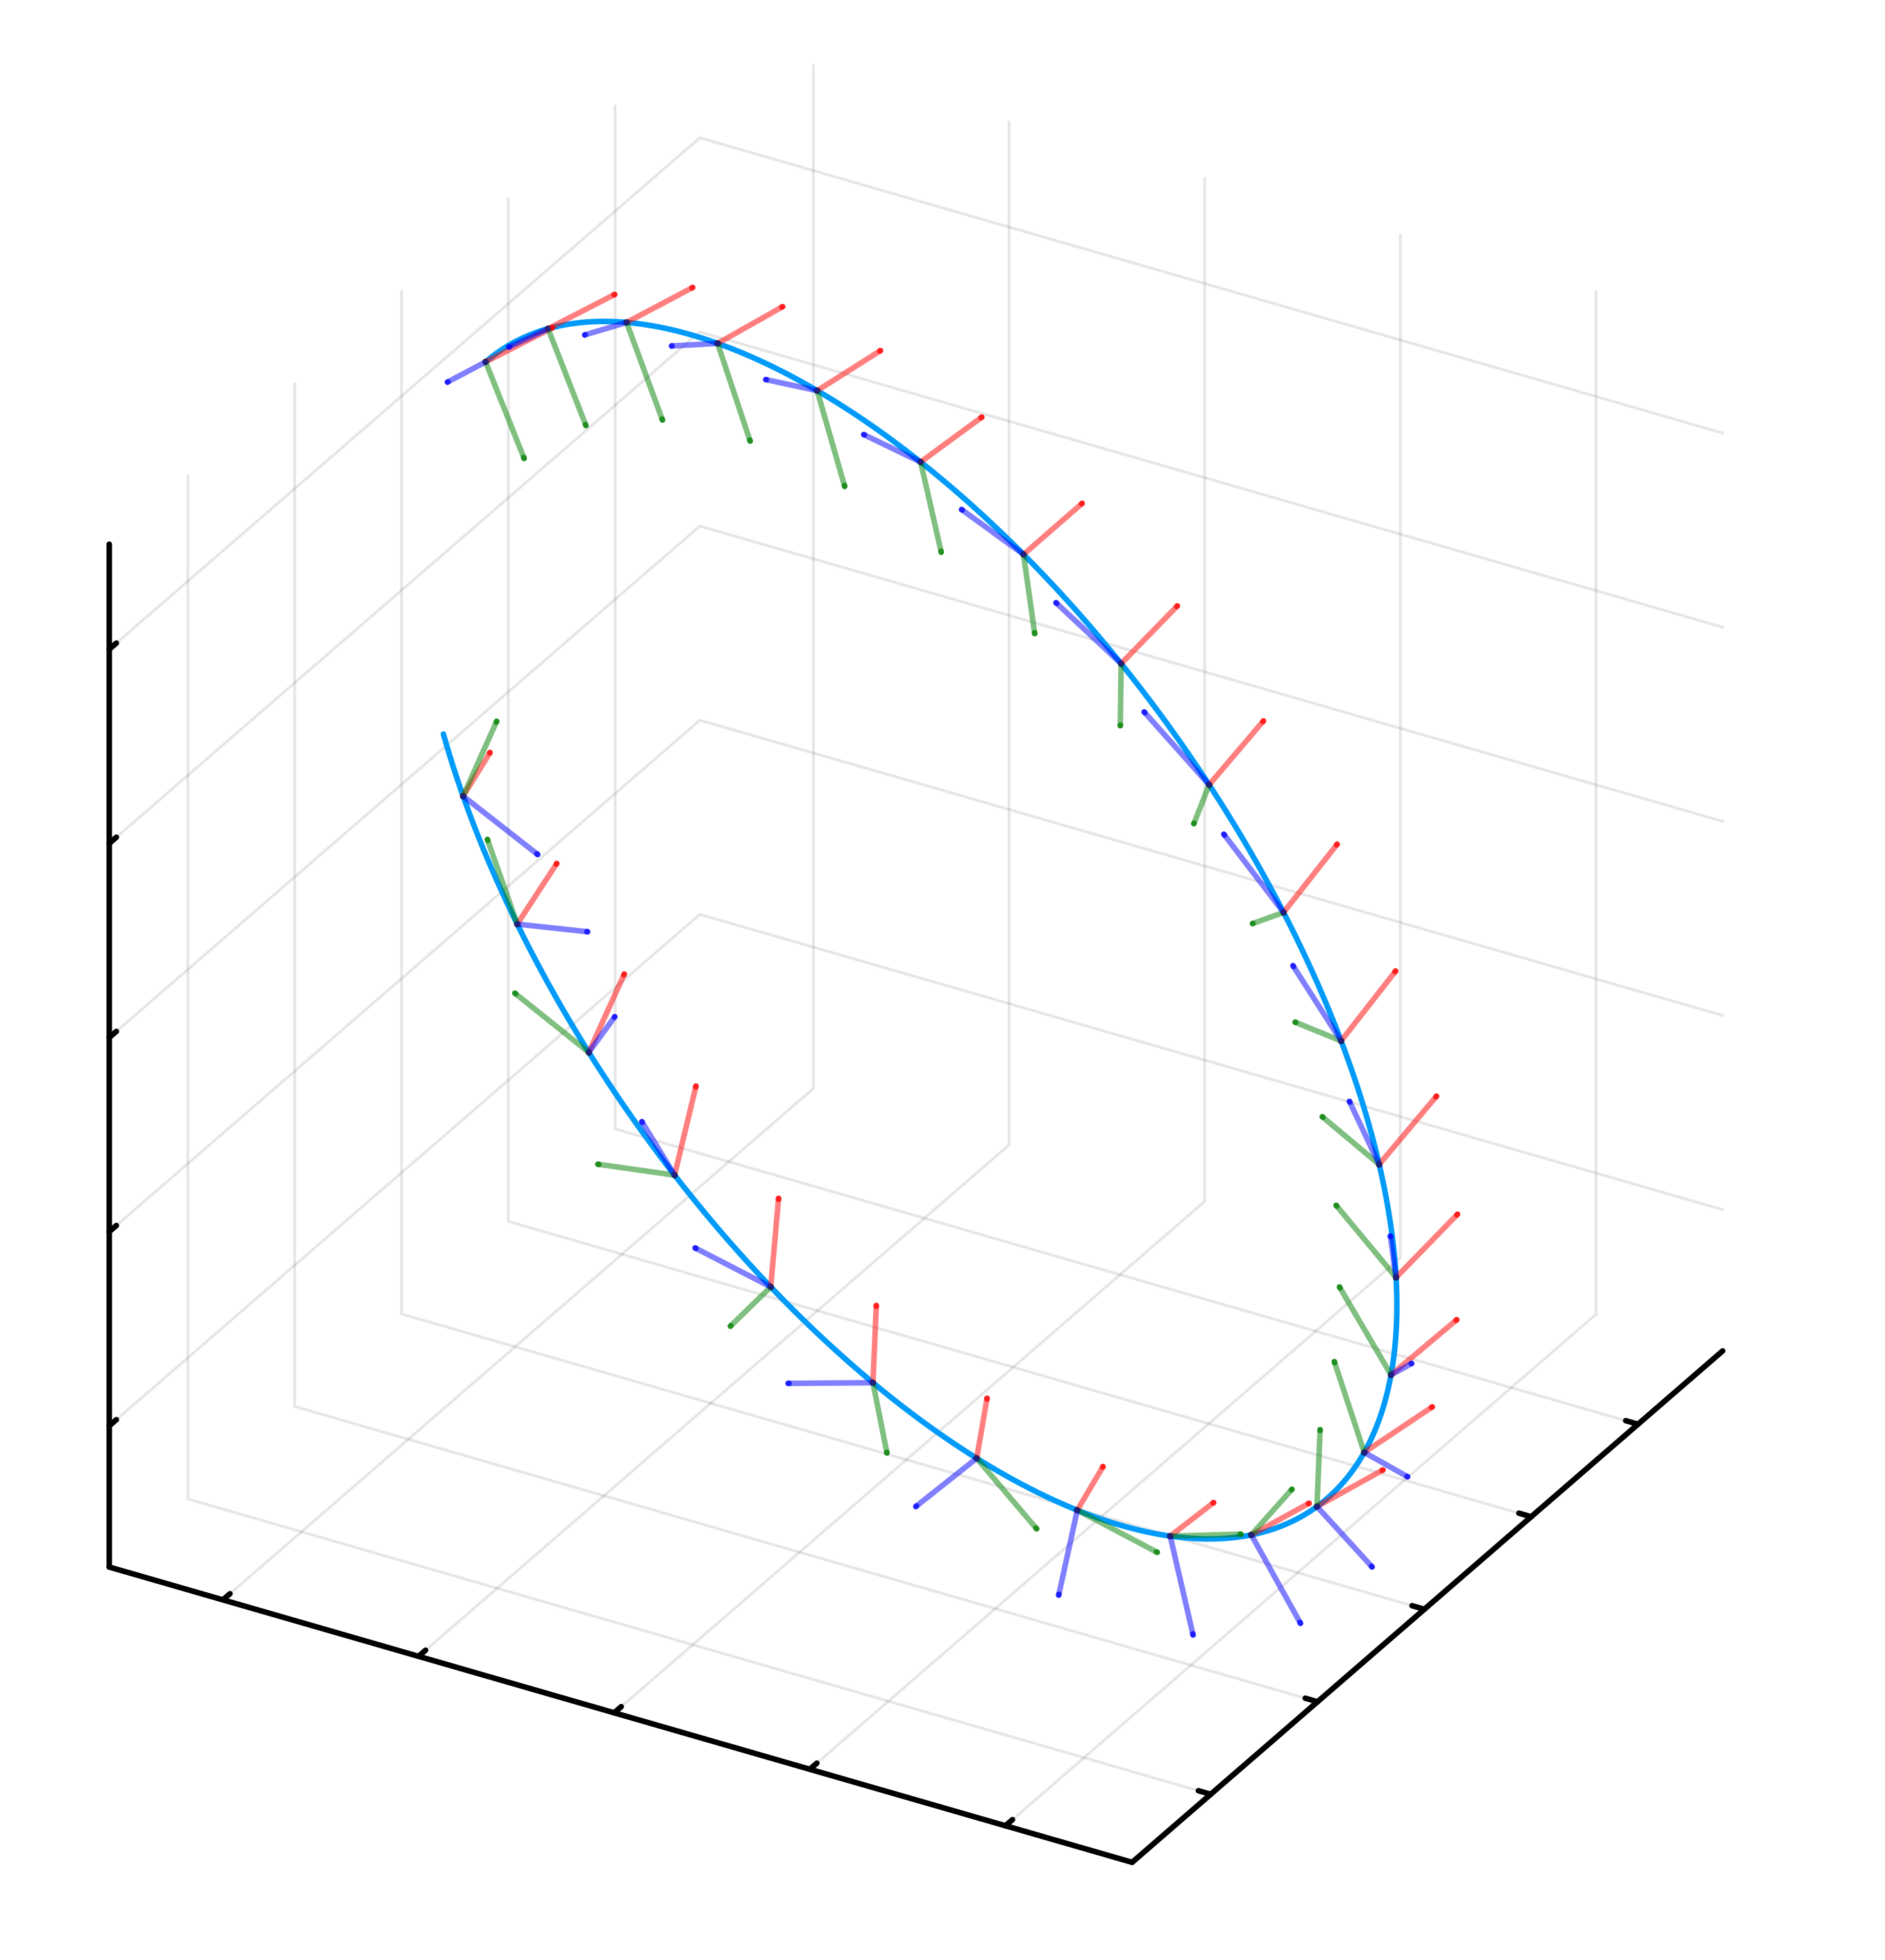
\includegraphics[width=4cm]{images/dist_orbit_0s_to_5100s.png}
		\caption{Evolution of $\mathcal{F}_{B}$}
		\label{fig:orbit_dist}
	\end{subfigure}
	\caption{Body Frame Simulation (Uncontrolled)}
\end{figure}

\subsection{Pointing Error}

In controlling a Nadir pointing spacecraft it is not $q_B$ or $q_L$ that is of interest, but the relative rotation between the two $q_{B/L}$. With a quaternion based model, this is extremely easy to calculate \ref{eqn:q_b_lvlh}. Similarly the angular velocity of the satellite must be expressed in body coordinated relative to $\mathcal{F}_L$ \ref{eqn:w_b_lvlh}.

\begin{equation}
	q_{B/L} = q_B \otimes q_L^{-1}
	\label{eqn:q_b_lvlh}
\end{equation}

\begin{equation}
	\omega_{B/L}^B = \omega_{B/I}^{B} - q_{B/L} \otimes \omega_{L/I}^{L} \otimes q_{b/L}^{-1}
	\label{eqn:w_b_lvlh}
\end{equation}

Plotting the pointing error for the previous simulation shows that the angular velocity from $\mathcal{F}_L$ rotating away from $\mathcal{F}_B$ from the perspective of $\mathcal{F}_B$ is now included in the results.

\begin{figure}[h]
	\centering
	\includegraphics[width=10cm]{images/dist_attitude_lvlh}
	\caption{Evolution of $q_{B/L}$ (Uncontrolled)}
\end{figure}

\section{PD Control}

A Proportional-Derivative (PD) controller was implemented based on the error quaternion \ref{eqn:pd}. 

\begin{equation}
	u = -k_d * \omega_{B/L}^{B} - k_p * q_{B/L}
	\label{eqn:pd}
\end{equation}

The gains $k_p = 1$ and $k_d = 10$ where found to addiquatley stabilize the satellite in under one orbit. Figures \ref{fig:quat_pd_perfect} and \ref{fig:orbit_pd_perfect} satellite aligning its body axes to the rotating LVLH frame under the pressence of disturbances. There is a slight steady state error as the controller contains no intgral action.

\begin{figure}[H]
\centering
	\begin{subfigure}[b]{0.6\textwidth}
		\centering
		\includegraphics[width=8cm]{images/pd_perfect_attitude_lvlh.png}
		\caption{Evolution of $q_{B/L}$}
		\label{fig:quat_pd_perfect}
	\end{subfigure}
	\begin{subfigure}[b]{0.3\textwidth}
		\centering
		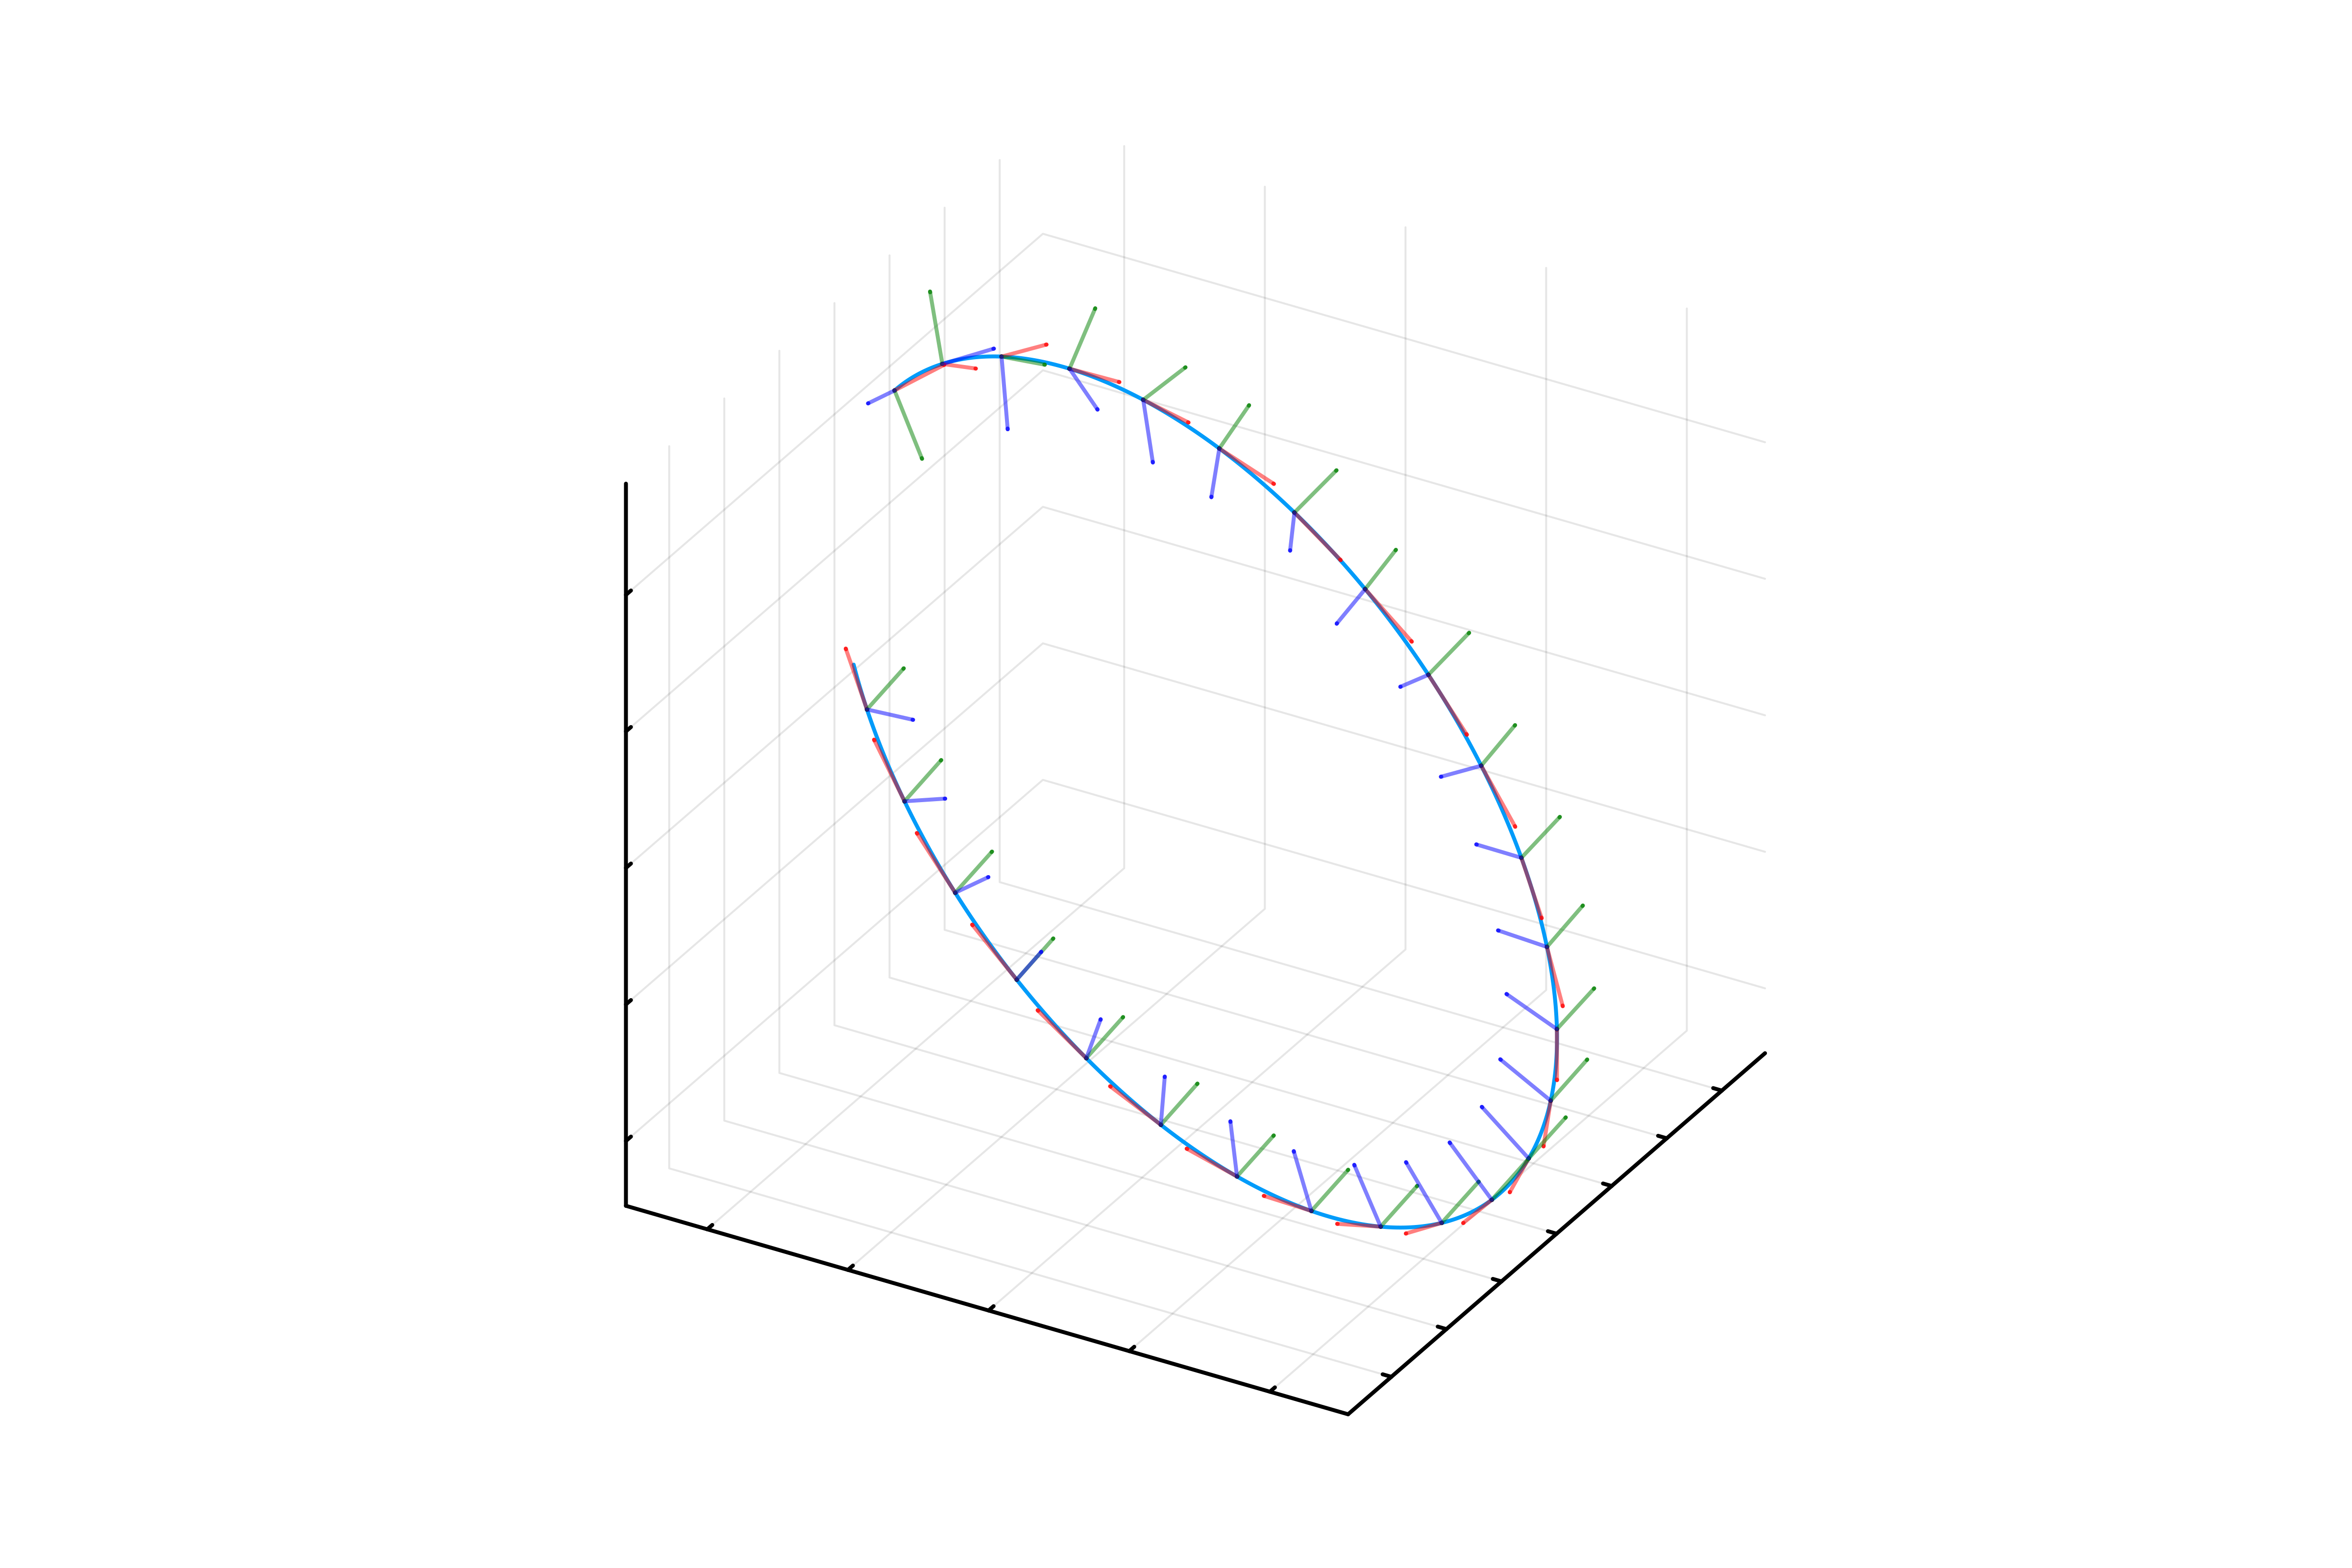
\includegraphics[width=4cm]{images/pd_perfect_orbit_0s_to_5100s.png}
		\caption{Evolution of $\mathcal{F}_{B}$}
		\label{fig:orbit_pd_perfect}
	\end{subfigure}
	\caption{Body Frame Simulation PD Control}
\end{figure}

The PD controller cannot cope with addition of white noise with a standard deviation of \SI{0.1}{\degree} to all body axis attitude measurements, and a bias of $\omega_{bias} = [\begin{matrix} 0.2 & -0.1 & 0.15\end{matrix}] \SI{}{\degree/\second}$ to the body rate measurments. As seen in figures \ref{fig:quat_pd_noise} and \ref{fig:orbit_pd_noise}, the peformance of the LVLH tracking suffers greatly and the an oscillation in the attitiude perisits through the orbit.

\begin{figure}[H]
\centering
	\begin{subfigure}[b]{0.6\textwidth}
		\centering
		\includegraphics[width=8cm]{images/pd_noise_attitude_lvlh.png}
		\caption{Evolution of $q_{B/L}$}
		\label{fig:quat_pd_noise}
	\end{subfigure}
	\begin{subfigure}[b]{0.3\textwidth}
		\centering
		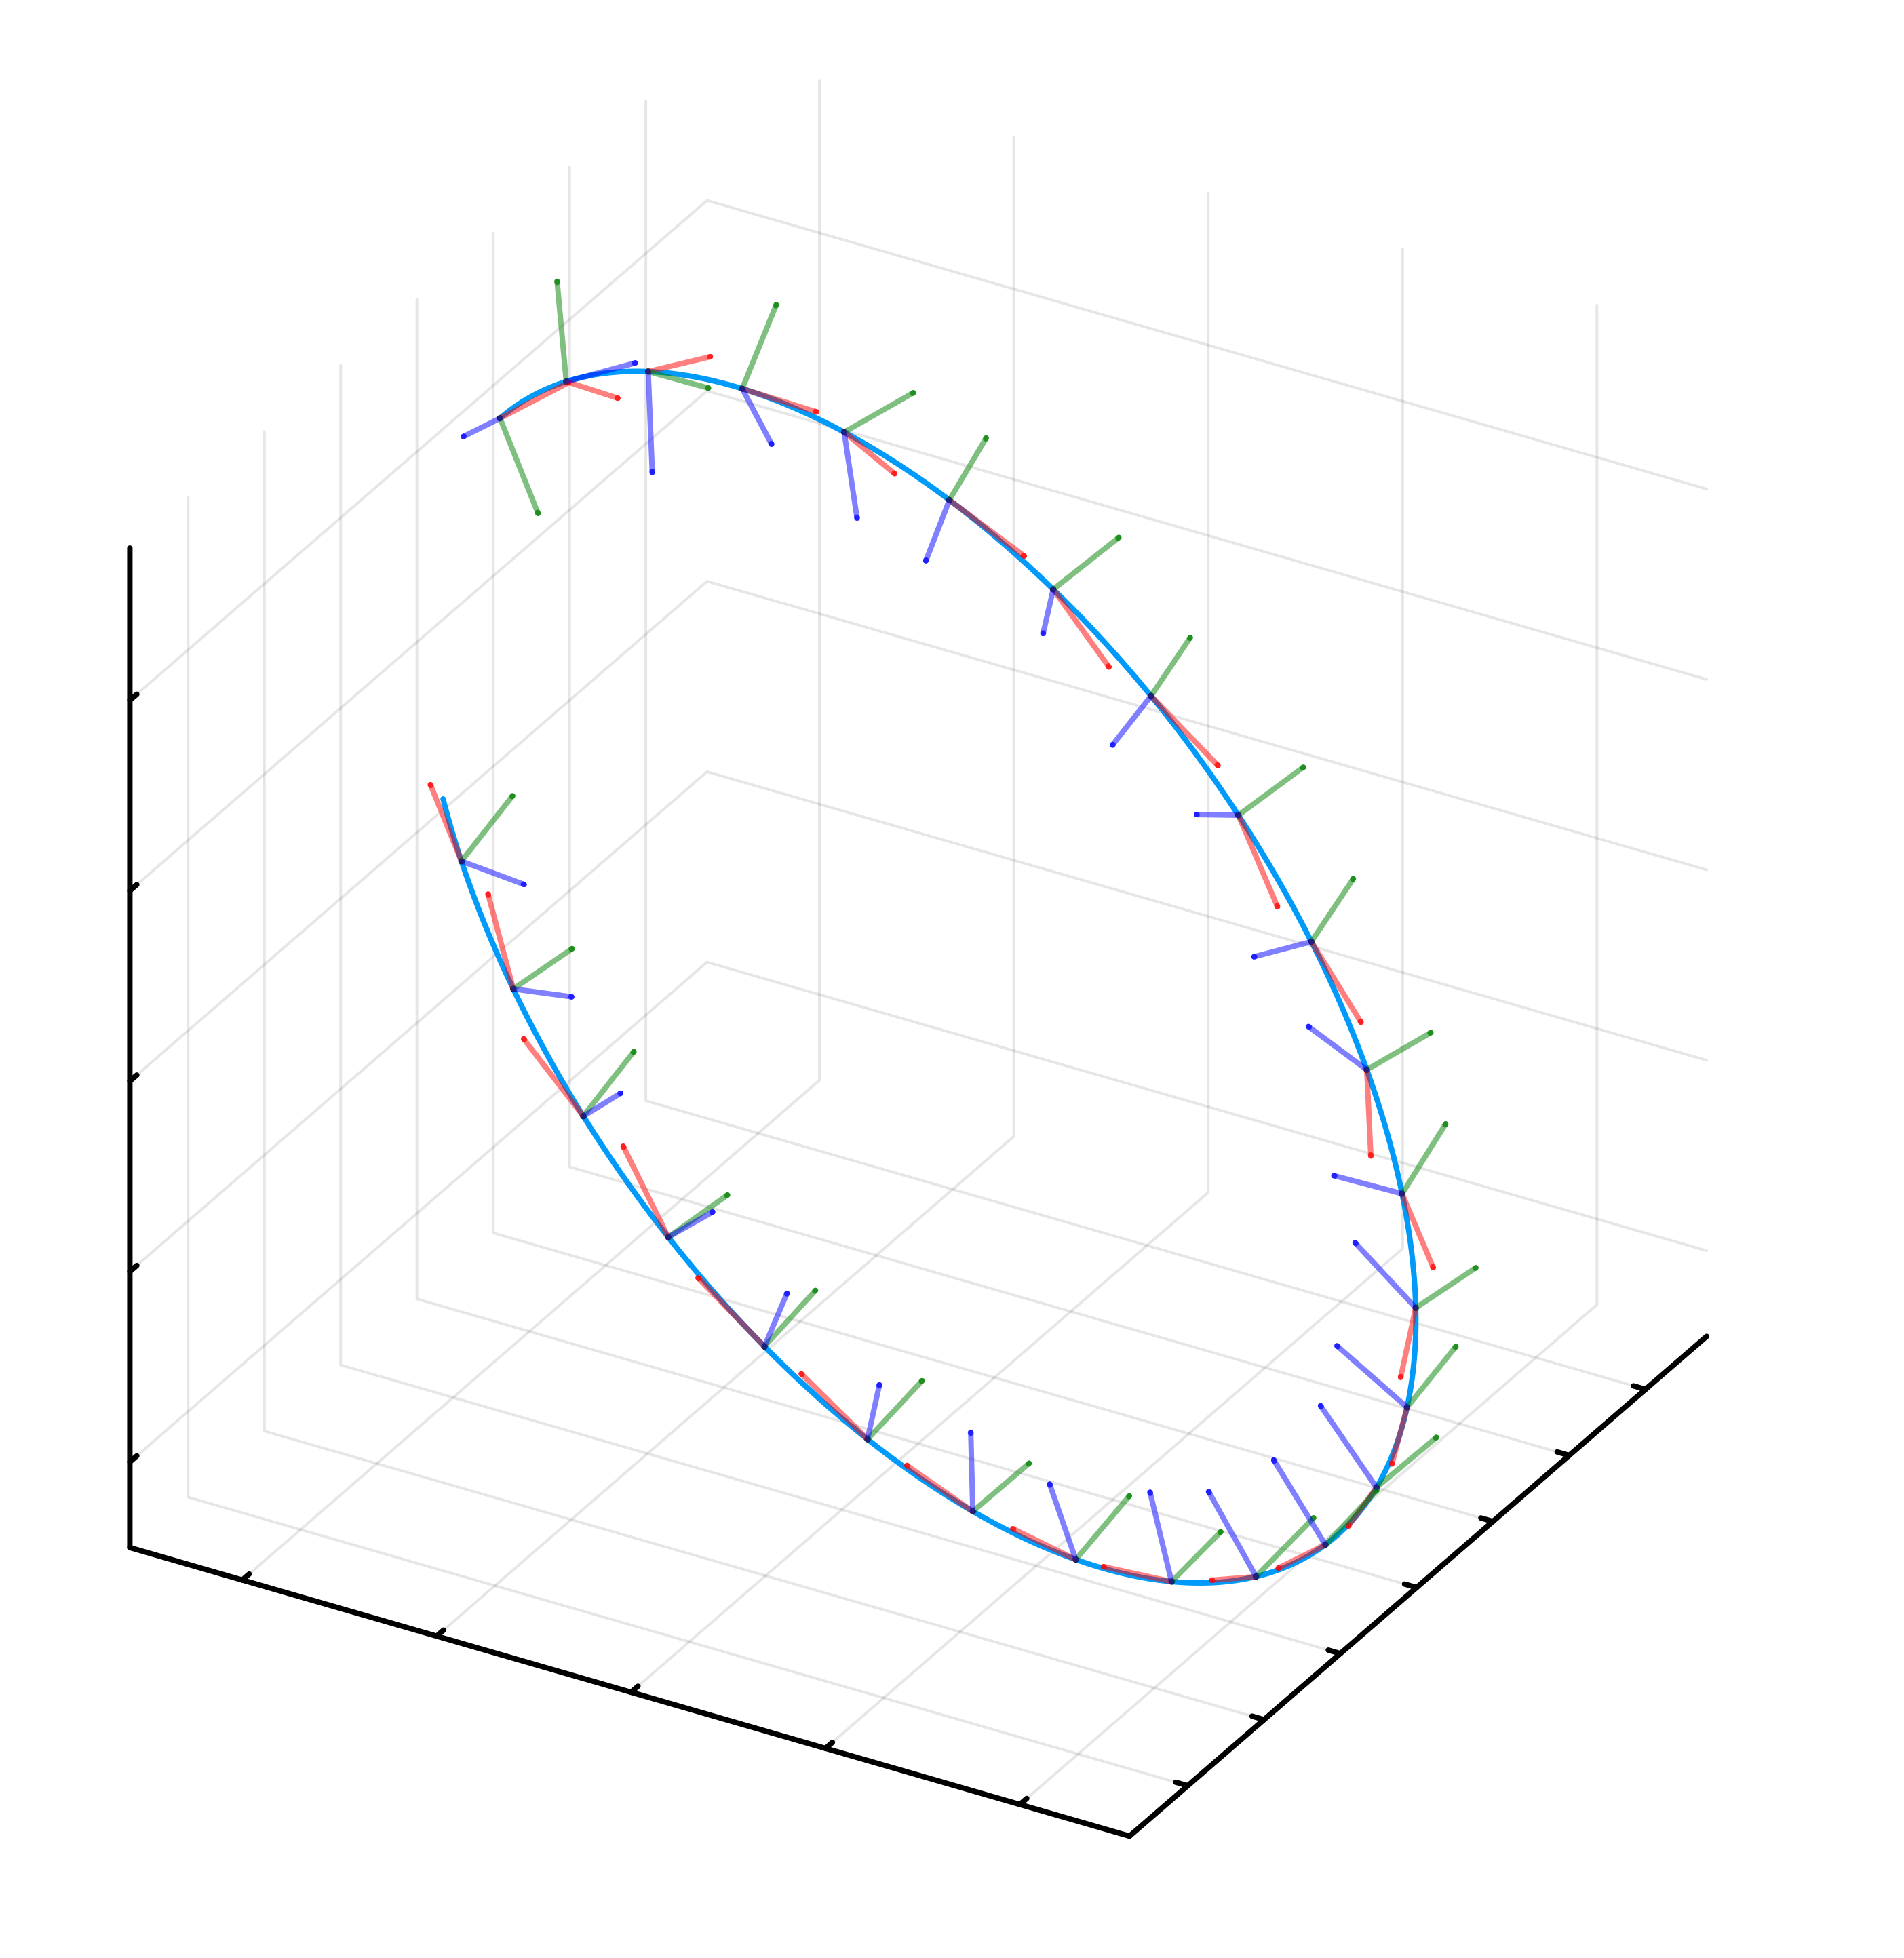
\includegraphics[width=4cm]{images/pd_noise_orbit_0s_to_5100s.png}
		\caption{Evolution of $\mathcal{F}_{B}$}
		\label{fig:orbit_pd_noise}
	\end{subfigure}
	\caption{Body Frame Simulation PD Control + Noise}
\end{figure}



\end{document}
